% =============================================================================
% Janus Lab — Lecture 01: RISC-V CPU Introduction
% Covers: ISA, micro-architecture, and lab module overview
% Compile with: pdflatex 01_cpu_intro.tex  (twice for ToC/overlays)
% =============================================================================
\documentclass[aspectratio=169,10pt]{beamer}

% ── Theme ────────────────────────────────────────────────────────────────────
\usetheme{Madrid}
\usecolortheme{beaver}
\setbeamertemplate{navigation symbols}{}
\setbeamertemplate{footline}[frame number]
\setbeamerfont{frametitle}{size=\normalsize,series=\bfseries}

% ── Packages ─────────────────────────────────────────────────────────────────
\usepackage{booktabs}
\usepackage{array}
\usepackage{colortbl}
\usepackage{listings}
\usepackage{tikz}
\usepackage{pgf}
\usepackage{xcolor}
\usepackage{fontawesome5}
\usepackage{amsmath}
\usepackage{graphicx}
\usepackage{microtype}

\usetikzlibrary{arrows.meta, shapes.geometric, positioning, fit, backgrounds, calc}

% ── Listing style for Verilog ────────────────────────────────────────────────
\lstdefinelanguage{Verilog}{
  morekeywords={module,endmodule,input,output,wire,reg,always,posedge,
    negedge,begin,end,if,else,case,endcase,assign,parameter,localparam,
    initial,default,integer},
  sensitive=true,
  morecomment=[l]{//},
  morecomment=[s]{/*}{*/},
  morestring=[b]"
}
\lstset{
  language=Verilog,
  basicstyle=\ttfamily\scriptsize,
  keywordstyle=\color{blue!70!black}\bfseries,
  commentstyle=\color{gray}\itshape,
  stringstyle=\color{red!70!black},
  backgroundcolor=\color{black!4},
  frame=single,
  framerule=0.4pt,
  xleftmargin=6pt,
  xrightmargin=6pt,
  breaklines=true,
  tabsize=4,
  showstringspaces=false,
}

% ── Colour palette ───────────────────────────────────────────────────────────
\definecolor{janusblue}{RGB}{25,70,140}
\definecolor{janusred}{RGB}{180,30,30}
\definecolor{janusgray}{RGB}{90,90,90}
\definecolor{stageIF}{RGB}{198,224,180}
\definecolor{stageID}{RGB}{180,198,231}
\definecolor{stageEX}{RGB}{255,217,102}
\definecolor{stageMEM}{RGB}{248,203,173}
\definecolor{stageWB}{RGB}{217,173,248}
\definecolor{pipeboxbg}{RGB}{245,245,245}

% ── Title info ───────────────────────────────────────────────────────────────
\title[Janus Lab -- CPU Intro]{Janus Lab: Implementing a Tiny RISC-V CPU}
\subtitle{Lecture 01 --- ISA, Microarchitecture, and Module Overview}
\author{Janus Lab}
\date{\today}
\institute{CPU Design and Implementation}

% =============================================================================
\begin{document}
% =============================================================================

% ── Title frame ──────────────────────────────────────────────────────────────
\begin{frame}
  \titlepage
\end{frame}

% ── Outline ──────────────────────────────────────────────────────────────────
\begin{frame}{Outline}
  \tableofcontents
\end{frame}

% =============================================================================
\section{Why RISC-V?}
% =============================================================================

\begin{frame}{Why RISC-V?}
  \begin{columns}[T]
    \begin{column}{0.55\textwidth}
      \textbf{RISC-V is an open, royalty-free ISA standard}
      \vspace{0.5em}
      \begin{itemize}
        \item Designed at UC Berkeley (2010); now governed by RISC-V International
        \item Clean, minimal base ISA with optional standard extensions
        \item Widely adopted in academia, industry, and silicon
        \item Excellent open-source toolchain: GCC, LLVM, Spike, QEMU
      \end{itemize}
      \vspace{0.8em}
      \textbf{Why it is ideal for this lab}
      \begin{itemize}
        \item \texttt{RV32I} base has only \textbf{47 instructions} --- manageable scope
        \item Fixed 32-bit instruction encoding --- no variable-length decode complexity
        \item Regular opcode/funct fields make control logic systematic
        \item Large community resources, reference implementations, test suites
      \end{itemize}
    \end{column}
    \begin{column}{0.40\textwidth}
      \begin{block}{RISC-V Extension Naming}
        \centering
        \renewcommand{\arraystretch}{1.3}
        \begin{tabular}{ll}
          \toprule
          Ext. & Meaning \\
          \midrule
          \texttt{RV32\textbf{I}} & Base integer (this lab) \\
          \texttt{M} & Multiply / divide \\
          \texttt{A} & Atomic operations \\
          \texttt{F} & Single-precision FP \\
          \texttt{D} & Double-precision FP \\
          \texttt{C} & Compressed (16-bit) \\
          \texttt{Zicsr} & CSR instructions \\
          \bottomrule
        \end{tabular}
      \end{block}
      \vspace{0.4em}
      \small
      \textit{``G'' = IMAFDZicsr\_Zifencei (general-purpose)}
    \end{column}
  \end{columns}
\end{frame}

% =============================================================================
\section{RV32I Instruction Set Architecture}
% =============================================================================

\begin{frame}{RV32I --- Programmer-Visible State}
  \begin{columns}[T]
    \begin{column}{0.48\textwidth}
      \textbf{Registers}
      \begin{itemize}
        \item 32 general-purpose registers: \texttt{x0}--\texttt{x31}
        \item Each register is \textbf{32 bits} wide
        \item \texttt{x0} is \emph{hardwired to zero} --- reads always return 0, writes are ignored
        \item No dedicated flags register (branch conditions computed on-the-fly)
        \item Program Counter (\texttt{pc}): 32-bit, not directly accessible
      \end{itemize}
      \vspace{0.5em}
      \textbf{Memory}
      \begin{itemize}
        \item Byte-addressable flat address space ($2^{32}$ bytes)
        \item Little-endian byte ordering
        \item Natural alignment strongly recommended (required in this lab)
      \end{itemize}
    \end{column}
    \begin{column}{0.48\textwidth}
      \begin{block}{ABI Register Aliases (RISC-V calling convention)}
        \renewcommand{\arraystretch}{1.1}
        \scriptsize
        \begin{tabular}{lll}
          \toprule
          Reg & ABI Name & Role \\
          \midrule
          \texttt{x0}  & \texttt{zero} & Always zero \\
          \texttt{x1}  & \texttt{ra}   & Return address \\
          \texttt{x2}  & \texttt{sp}   & Stack pointer \\
          \texttt{x3}  & \texttt{gp}   & Global pointer \\
          \texttt{x5--7}  & \texttt{t0--2} & Temporaries \\
          \texttt{x8}  & \texttt{s0/fp} & Saved / frame ptr \\
          \texttt{x10--11} & \texttt{a0--1} & Args / return vals \\
          \texttt{x12--17} & \texttt{a2--7} & Arguments \\
          \texttt{x18--27} & \texttt{s2--11} & Saved registers \\
          \texttt{x28--31} & \texttt{t3--6} & Temporaries \\
          \bottomrule
        \end{tabular}
      \end{block}
    \end{column}
  \end{columns}
\end{frame}

% ── Instruction encoding ──────────────────────────────────────────────────────
\begin{frame}{RV32I Instruction Encoding Formats}
  \small
  All RV32I instructions are \textbf{exactly 32 bits} wide. Six encoding formats share a common opcode field at bits [6:0].
  \vspace{0.6em}

  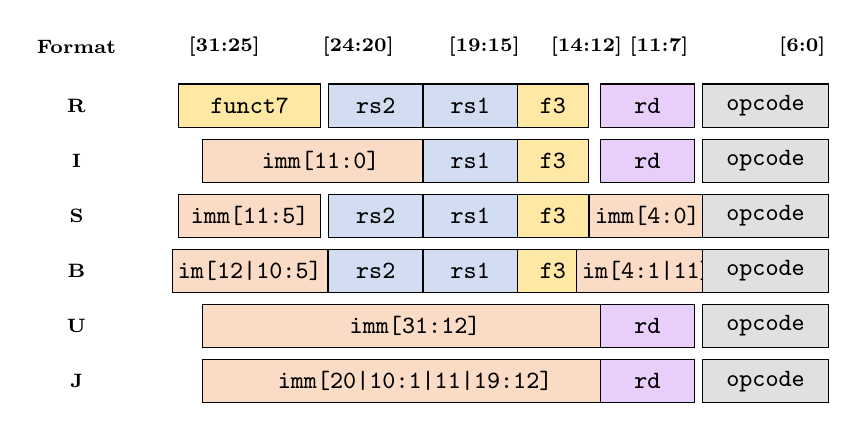
\begin{tikzpicture}[
    box/.style={draw, minimum height=0.55cm, minimum width=#1, font=\ttfamily\scriptsize, inner sep=2pt},
    lbl/.style={font=\scriptsize\bfseries}
  ]
    \newcommand{\bitrow}[9]{%
      \node[box=1.2cm, fill=black!10] {#2}; % 31:25
      \node[box=0.9cm, fill=white]    [right=0pt of \tikzlastnode] {#3};
      \node[box=0.9cm, fill=white]    [right=0pt of \tikzlastnode] {#4};
      \node[box=0.7cm, fill=black!10] [right=0pt of \tikzlastnode] {#5};
      \node[box=1.4cm, fill=white]    [right=0pt of \tikzlastnode] {#6};
      \node[box=0.9cm, fill=black!10] [right=0pt of \tikzlastnode] {#7};
      % label on left
    }

    % Column headers
    \node[lbl] at (0,0) {Format};
    \node[lbl, anchor=west] at (1.3,0) {[31:25]};
    \node[lbl, anchor=west] at (3.0,0) {[24:20]};
    \node[lbl, anchor=west] at (4.6,0) {[19:15]};
    \node[lbl, anchor=west] at (5.9,0) {[14:12]};
    \node[lbl, anchor=west] at (6.9,0) {[11:7]};
    \node[lbl, anchor=west] at (8.8,0) {[6:0]};

    % R-type
    \node[lbl] at (0,-0.75) {R};
    \node[box=1.8cm, fill=stageEX!60]  at (2.2,-0.75) {\small funct7};
    \node[box=1.2cm, fill=stageID!60]  at (3.8,-0.75) {\small rs2};
    \node[box=1.2cm, fill=stageID!60]  at (5.0,-0.75) {\small rs1};
    \node[box=0.9cm, fill=stageEX!60]  at (6.05,-0.75){\small f3};
    \node[box=1.2cm, fill=stageWB!60]  at (7.25,-0.75){\small rd};
    \node[box=1.6cm, fill=black!12]    at (8.75,-0.75){\small opcode};

    % I-type
    \node[lbl] at (0,-1.45) {I};
    \node[box=3.0cm, fill=stageMEM!70] at (3.1,-1.45) {\small imm[11:0]};
    \node[box=1.2cm, fill=stageID!60]  at (5.0,-1.45) {\small rs1};
    \node[box=0.9cm, fill=stageEX!60]  at (6.05,-1.45){\small f3};
    \node[box=1.2cm, fill=stageWB!60]  at (7.25,-1.45){\small rd};
    \node[box=1.6cm, fill=black!12]    at (8.75,-1.45){\small opcode};

    % S-type
    \node[lbl] at (0,-2.15) {S};
    \node[box=1.8cm, fill=stageMEM!70] at (2.2,-2.15)  {\small imm[11:5]};
    \node[box=1.2cm, fill=stageID!60]  at (3.8,-2.15)  {\small rs2};
    \node[box=1.2cm, fill=stageID!60]  at (5.0,-2.15)  {\small rs1};
    \node[box=0.9cm, fill=stageEX!60]  at (6.05,-2.15) {\small f3};
    \node[box=1.2cm, fill=stageMEM!70] at (7.25,-2.15) {\small imm[4:0]};
    \node[box=1.6cm, fill=black!12]    at (8.75,-2.15) {\small opcode};

    % B-type
    \node[lbl] at (0,-2.85) {B};
    \node[box=1.8cm, fill=stageMEM!70] at (2.2,-2.85)  {\small im[12|10:5]};
    \node[box=1.2cm, fill=stageID!60]  at (3.8,-2.85)  {\small rs2};
    \node[box=1.2cm, fill=stageID!60]  at (5.0,-2.85)  {\small rs1};
    \node[box=0.9cm, fill=stageEX!60]  at (6.05,-2.85) {\small f3};
    \node[box=1.2cm, fill=stageMEM!70] at (7.25,-2.85) {\small im[4:1|11]};
    \node[box=1.6cm, fill=black!12]    at (8.75,-2.85) {\small opcode};

    % U-type
    \node[lbl] at (0,-3.55) {U};
    \node[box=5.4cm, fill=stageMEM!70] at (4.3,-3.55)  {\small imm[31:12]};
    \node[box=1.2cm, fill=stageWB!60]  at (7.25,-3.55) {\small rd};
    \node[box=1.6cm, fill=black!12]    at (8.75,-3.55) {\small opcode};

    % J-type
    \node[lbl] at (0,-4.25) {J};
    \node[box=5.4cm, fill=stageMEM!70] at (4.3,-4.25)  {\small imm[20|10:1|11|19:12]};
    \node[box=1.2cm, fill=stageWB!60]  at (7.25,-4.25) {\small rd};
    \node[box=1.6cm, fill=black!12]    at (8.75,-4.25) {\small opcode};
  \end{tikzpicture}

  \vspace{0.4em}
  \small
  \textbf{Key observation:} \texttt{rs1}, \texttt{rs2}, and \texttt{rd} always occupy the same bit positions across all formats --- simplifying the register file read/write logic.
\end{frame}

% ── Instruction table ─────────────────────────────────────────────────────────
\begin{frame}{RV32I Instruction Set (47 Instructions)}
  \renewcommand{\arraystretch}{1.2}
  \small
  \begin{tabular}{>{\bfseries}l p{9.5cm}}
    \toprule
    Type & Instructions \\
    \midrule
    R & \texttt{ADD SUB SLL SLT SLTU XOR SRL SRA OR AND} \\
    \rowcolor{black!5}
    I (arith) & \texttt{ADDI SLTI SLTIU XORI ORI ANDI SLLI SRLI SRAI} \\
    I (load)  & \texttt{LB LH LW LBU LHU} \\
    \rowcolor{black!5}
    S         & \texttt{SB SH SW} \\
    B         & \texttt{BEQ BNE BLT BGE BLTU BGEU} \\
    \rowcolor{black!5}
    U         & \texttt{LUI AUIPC} \\
    J         & \texttt{JAL JALR} \\
    \midrule
    \textit{Excluded} & \texttt{FENCE ECALL EBREAK} \quad (Phase 3 stretch goals) \\
    \bottomrule
  \end{tabular}

  \vspace{0.8em}
  \begin{columns}[T]
    \begin{column}{0.45\textwidth}
      \textbf{Opcode map (bits [6:0])}\\[0.3em]
      \scriptsize
      \begin{tabular}{ll}
        \texttt{0110011} & R-type \\
        \texttt{0010011} & I-type arithmetic \\
        \texttt{0000011} & Loads \\
        \texttt{0100011} & Stores \\
        \texttt{1100011} & Branches \\
        \texttt{0110111} & LUI \\
        \texttt{0010111} & AUIPC \\
        \texttt{1101111} & JAL \\
        \texttt{1100111} & JALR \\
      \end{tabular}
    \end{column}
    \begin{column}{0.50\textwidth}
      \textbf{funct3 / funct7 sub-decode (R-type)}\\[0.3em]
      \scriptsize
      \begin{tabular}{lll}
        \texttt{funct3} & \texttt{funct7} & Instr \\
        \hline
        \texttt{000} & \texttt{0000000} & ADD \\
        \texttt{000} & \texttt{0100000} & SUB \\
        \texttt{101} & \texttt{0000000} & SRL \\
        \texttt{101} & \texttt{0100000} & SRA \\
        \texttt{001} & \texttt{0000000} & SLL \\
        \texttt{010} & \texttt{0000000} & SLT \\
        \texttt{011} & \texttt{0000000} & SLTU \\
      \end{tabular}
    \end{column}
  \end{columns}
\end{frame}

% ── Notable instructions ──────────────────────────────────────────────────────
\begin{frame}{Notable Instructions to Understand Well}
  \begin{columns}[T]
    \begin{column}{0.48\textwidth}
      \begin{block}{\texttt{LUI} --- Load Upper Immediate}
        \texttt{rd = imm[31:12] << 12}\\[0.3em]
        Places a 20-bit immediate into the upper 20 bits of \texttt{rd}, clearing the lower 12 bits.
        Used together with \texttt{ADDI} to build arbitrary 32-bit constants.\\[0.3em]
        \textbf{Datapath note:} ALU receives the immediate via \texttt{alu\_src=1}; operation is \textit{pass-through} (no rs1 involvement).
      \end{block}
      \vspace{0.5em}
      \begin{block}{\texttt{AUIPC} --- Add Upper Immediate to PC}
        \texttt{rd = pc + (imm[31:12] << 12)}\\[0.3em]
        PC-relative addressing. Used to synthesise position-independent code and to form jump targets beyond the 12-bit JALR offset range.
      \end{block}
    \end{column}
    \begin{column}{0.48\textwidth}
      \begin{block}{\texttt{JAL} --- Jump and Link}
        \texttt{rd = pc+4; pc = pc + imm}\\[0.3em]
        21-bit signed PC-relative offset ($\pm$1 MB range). Saves return address. Used for function calls.
      \end{block}
      \vspace{0.5em}
      \begin{block}{\texttt{JALR} --- Jump and Link Register}
        \texttt{rd = pc+4; pc = (rs1 + imm) \& \textasciitilde1}\\[0.3em]
        Indirect jump through register. LSB of target is forced to 0. Used for function returns (\texttt{jalr x0, 0(ra)}) and computed jumps.
      \end{block}
      \vspace{0.5em}
      \begin{block}{Branch Instructions}
        Signed: \texttt{BEQ BNE BLT BGE}\\
        Unsigned: \texttt{BLTU BGEU}\\[0.3em]
        All branches are PC-relative with a 13-bit signed offset ($\pm$4 KB range).
      \end{block}
    \end{column}
  \end{columns}
\end{frame}

% =============================================================================
\section{Microarchitecture Overview}
% =============================================================================

\begin{frame}{Lab Structure: Three Phases}
  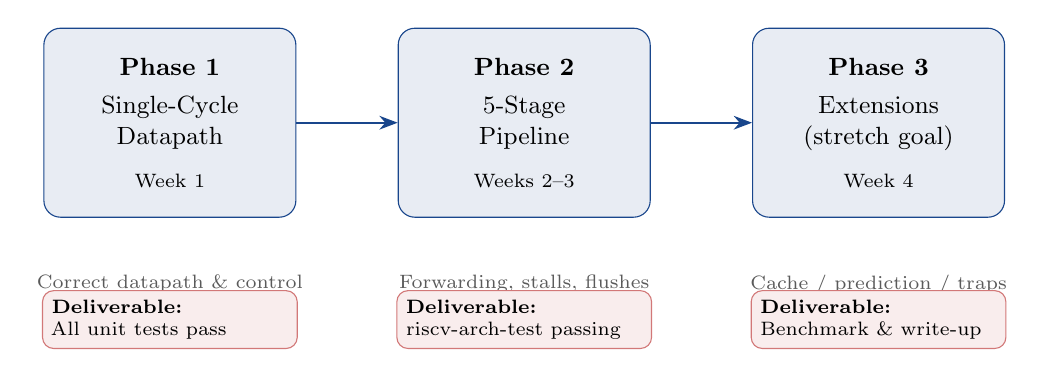
\begin{tikzpicture}[
    phase/.style={draw=janusblue, fill=janusblue!10, rounded corners=6pt,
                  minimum width=3.2cm, minimum height=2.4cm, align=center,
                  font=\small},
    arrow/.style={-Stealth, thick, janusblue},
    label/.style={font=\scriptsize, text=janusgray}
  ]
    \node[phase] (p1) at (0,0) {\textbf{Phase 1}\\[0.3em]Single-Cycle\\Datapath\\[0.5em]\scriptsize Week 1};
    \node[phase] (p2) at (4.5,0) {\textbf{Phase 2}\\[0.3em]5-Stage\\Pipeline\\[0.5em]\scriptsize Weeks 2--3};
    \node[phase] (p3) at (9.0,0) {\textbf{Phase 3}\\[0.3em]Extensions\\(stretch goal)\\[0.5em]\scriptsize Week 4};

    \draw[arrow] (p1.east) -- (p2.west);
    \draw[arrow] (p2.east) -- (p3.west);

    \node[label, below=0.6cm of p1] {Correct datapath \& control};
    \node[label, below=0.6cm of p2] {Forwarding, stalls, flushes};
    \node[label, below=0.6cm of p3] {Cache / prediction / traps};

    % Deliverable callouts
    \node[draw=janusred!60, fill=janusred!8, rounded corners=4pt,
          font=\scriptsize, text width=3.0cm, align=left]
      at (0,-2.5) {\textbf{Deliverable:}\\All unit tests pass};
    \node[draw=janusred!60, fill=janusred!8, rounded corners=4pt,
          font=\scriptsize, text width=3.0cm, align=left]
      at (4.5,-2.5) {\textbf{Deliverable:}\\riscv-arch-test passing};
    \node[draw=janusred!60, fill=janusred!8, rounded corners=4pt,
          font=\scriptsize, text width=3.0cm, align=left]
      at (9.0,-2.5) {\textbf{Deliverable:}\\Benchmark \& write-up};
  \end{tikzpicture}
\end{frame}

% ── Single-cycle datapath ────────────────────────────────────────────────────
\begin{frame}{Phase 1: Single-Cycle Datapath}
  \begin{columns}[T]
    \begin{column}{0.52\textwidth}
      \textbf{Key idea:} Every instruction completes in \textbf{one clock cycle}.
      All five logical stages are combinational --- no pipeline registers between them.

      \vspace{0.8em}
      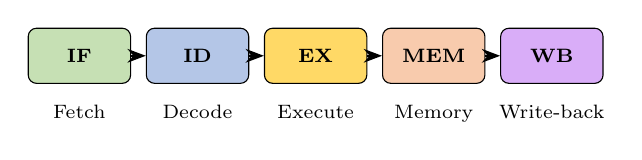
\begin{tikzpicture}[
        stage/.style={draw, fill=#1, minimum width=1.3cm, minimum height=0.7cm,
                      font=\bfseries\scriptsize, rounded corners=3pt},
        arr/.style={-Stealth, thick}
      ]
        \node[stage=stageIF]  (IF)  at (0,0)    {IF};
        \node[stage=stageID]  (ID)  at (1.5,0)  {ID};
        \node[stage=stageEX]  (EX)  at (3.0,0)  {EX};
        \node[stage=stageMEM] (MEM) at (4.5,0)  {MEM};
        \node[stage=stageWB]  (WB)  at (6.0,0)  {WB};
        \draw[arr] (IF)--(ID); \draw[arr] (ID)--(EX);
        \draw[arr] (EX)--(MEM); \draw[arr] (MEM)--(WB);
        \node[font=\scriptsize, below=0.15cm of IF]  {Fetch};
        \node[font=\scriptsize, below=0.15cm of ID]  {Decode};
        \node[font=\scriptsize, below=0.15cm of EX]  {Execute};
        \node[font=\scriptsize, below=0.15cm of MEM] {Memory};
        \node[font=\scriptsize, below=0.15cm of WB]  {Write-back};
      \end{tikzpicture}

      \vspace{0.8em}
      \textbf{Harvard architecture:}
      \begin{itemize}\small
        \item Separate instruction ROM (\texttt{imem}) and data RAM (\texttt{dmem})
        \item Both accessed in the same cycle --- no structural hazard
      \end{itemize}

      \vspace{0.5em}
      \textbf{Clock period} must accommodate the \emph{longest} combinational path (typically a load: imem $\to$ regfile $\to$ ALU $\to$ dmem $\to$ regfile).
    \end{column}
    \begin{column}{0.44\textwidth}
      \begin{block}{Control Signals}
        \renewcommand{\arraystretch}{1.1}
        \scriptsize
        \begin{tabular}{lp{3.8cm}}
          \toprule
          Signal & Meaning \\
          \midrule
          \texttt{reg\_write}  & Enable register file write \\
          \texttt{alu\_src}    & 0=rs2, 1=immediate \\
          \texttt{alu\_op[1:0]}& ALU operation class \\
          \texttt{mem\_read}   & Enable data memory read \\
          \texttt{mem\_write}  & Enable data memory write \\
          \texttt{mem\_to\_reg}& 0=ALU result, 1=mem data \\
          \texttt{branch}      & Conditional branch \\
          \texttt{jump}        & JAL / JALR \\
          \bottomrule
        \end{tabular}
      \end{block}
    \end{column}
  \end{columns}
\end{frame}

% ── 5-stage pipeline ─────────────────────────────────────────────────────────
\begin{frame}{Phase 2: 5-Stage Pipeline}
  \begin{center}
  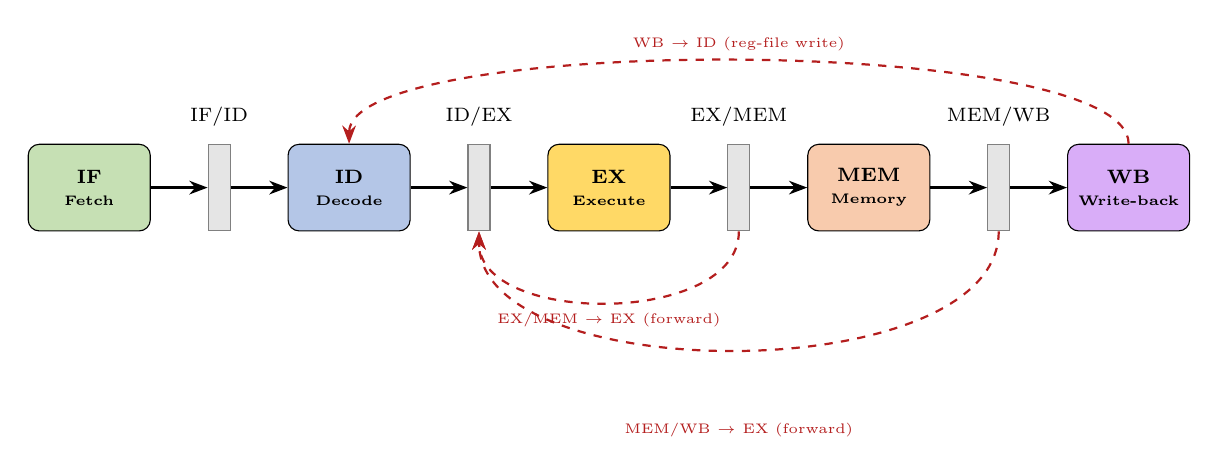
\begin{tikzpicture}[
    stage/.style={draw, fill=#1, minimum width=1.55cm, minimum height=1.1cm,
                  font=\bfseries\scriptsize, rounded corners=4pt, align=center},
    preg/.style={draw=black!50, fill=black!10, minimum width=0.28cm,
                 minimum height=1.1cm, font=\tiny, rotate=0},
    arr/.style={-Stealth, thick},
    fwd/.style={-Stealth, thick, dashed, janusred},
    lbl/.style={font=\scriptsize}
  ]
    % Stages
    \node[stage=stageIF]  (IF)  at (0,0)    {IF\\{\tiny Fetch}};
    \node[preg] (r1) at (1.65,0) {};
    \node[stage=stageID]  (ID)  at (3.3,0)  {ID\\{\tiny Decode}};
    \node[preg] (r2) at (4.95,0) {};
    \node[stage=stageEX]  (EX)  at (6.6,0)  {EX\\{\tiny Execute}};
    \node[preg] (r3) at (8.25,0) {};
    \node[stage=stageMEM] (MEM) at (9.9,0)  {MEM\\{\tiny Memory}};
    \node[preg] (r4) at (11.55,0) {};
    \node[stage=stageWB]  (WB)  at (13.2,0) {WB\\{\tiny Write-back}};

    % Register labels
    \node[lbl, above=0.1cm of r1] {\scriptsize IF/ID};
    \node[lbl, above=0.1cm of r2] {\scriptsize ID/EX};
    \node[lbl, above=0.1cm of r3] {\scriptsize EX/MEM};
    \node[lbl, above=0.1cm of r4] {\scriptsize MEM/WB};

    % Flow arrows
    \foreach \a/\b in {IF/r1, r1/ID, ID/r2, r2/EX, EX/r3, r3/MEM, MEM/r4, r4/WB}
      \draw[arr] (\a) -- (\b);

    % EX-EX forwarding arc
    \draw[fwd] (r3.south) .. controls +(0,-1.2) and +(0,-1.2) .. (r2.south)
      node[midway, below, font=\tiny, text=janusred] {EX/MEM $\to$ EX (forward)};

    % MEM-EX forwarding arc
    \draw[fwd] (r4.south) .. controls +(0,-2.0) and +(0,-2.0) .. (r2.south)
      node[midway, below, font=\tiny, yshift=-0.8cm, text=janusred] {MEM/WB $\to$ EX (forward)};

    % WB -> ID bypass (register file)
    \draw[fwd] (WB.north) .. controls +(0,1.4) and +(0,1.4) .. (ID.north)
      node[midway, above, font=\tiny, text=janusred] {WB $\to$ ID (reg-file write)};

  \end{tikzpicture}
  \end{center}

  \vspace{0.3em}
  \begin{columns}[T]
    \begin{column}{0.48\textwidth}
      \textbf{Pipeline registers} latch stage outputs each cycle.
      Each register can be independently \textit{stalled} (frozen) or \textit{flushed} (zeroed to NOP).
    \end{column}
    \begin{column}{0.48\textwidth}
      \textbf{Throughput goal:} one instruction completed per cycle in steady state (IPC $\approx$ 1), limited by hazards.
    \end{column}
  \end{columns}
\end{frame}

% ── Hazards ──────────────────────────────────────────────────────────────────
\begin{frame}{Pipeline Hazards}
  \begin{columns}[T]
    \begin{column}{0.32\textwidth}
      \begin{block}{Data Hazard --- Forwarding}
        \textbf{Problem:} Instruction in EX needs a value still in the pipeline.\\[0.4em]
        \textbf{Solution:} \texttt{forward\_unit} bypasses EX/MEM or MEM/WB result directly to ALU input.\\[0.4em]
        \textbf{Encoding:}\\
        \texttt{2'b00} = regfile\\
        \texttt{2'b01} = MEM/WB\\
        \texttt{2'b10} = EX/MEM (priority)
      \end{block}
    \end{column}
    \begin{column}{0.32\textwidth}
      \begin{block}{Load-Use Hazard --- Stall}
        \textbf{Problem:} Load result is not available until end of MEM; the very next instruction needs it.\\[0.4em]
        \textbf{Solution:} \texttt{hazard\_unit} freezes PC and IF/ID for one cycle; inserts NOP bubble into ID/EX.\\[0.4em]
        \textbf{Cost:} 1 stall cycle per load-use pair.
      \end{block}
    \end{column}
    \begin{column}{0.32\textwidth}
      \begin{block}{Control Hazard --- Flush}
        \textbf{Problem:} Branch/jump target is unknown until EX. Two instructions were already fetched.\\[0.4em]
        \textbf{Solution:} Predict-not-taken. On a taken branch or jump, flush IF/ID and ID/EX; redirect PC.\\[0.4em]
        \textbf{Cost:} 2-cycle penalty per taken branch.
      \end{block}
    \end{column}
  \end{columns}

  \vspace{0.8em}
  \begin{center}
  \small
  \begin{tabular}{lll}
    \toprule
    Hazard type & Detected by & Resolved by \\
    \midrule
    RAW (non-load) & \texttt{forward\_unit} & Forwarding --- no stall \\
    Load-use (RAW) & \texttt{hazard\_unit}  & 1-cycle stall + NOP bubble \\
    Branch/jump    & \texttt{hazard\_unit}  & 2-cycle flush \\
    \bottomrule
  \end{tabular}
  \end{center}
\end{frame}

% =============================================================================
\section{Module-by-Module Walkthrough}
% =============================================================================

\begin{frame}{Module Map}
  \begin{center}
  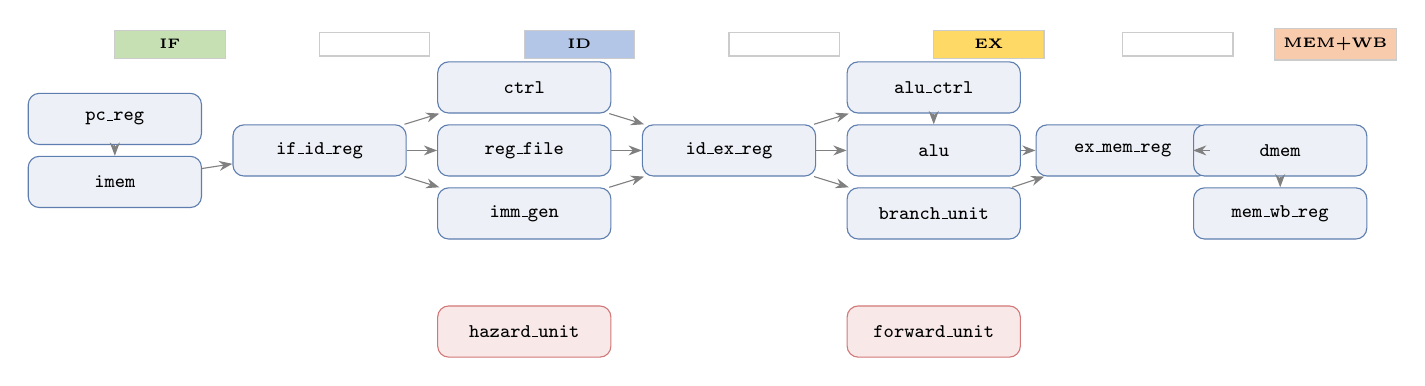
\begin{tikzpicture}[
    mod/.style={draw=janusblue!70, fill=janusblue!8, rounded corners=4pt,
                minimum width=2.2cm, minimum height=0.65cm, font=\scriptsize\ttfamily,
                align=center},
    container/.style={draw=black!40, fill=black!4, rounded corners=6pt, dashed},
    arr/.style={-Stealth, gray, thin}
  ]
    % cpu boundary
    \begin{scope}
      \node[mod] (pc)     at (0, 2.4)   {pc\_reg};
      \node[mod] (imem)   at (0, 1.6)   {imem};
      \node[mod] (ifid)   at (2.6, 2.0) {if\_id\_reg};
      \node[mod] (ctrl)   at (5.2, 2.8) {ctrl};
      \node[mod] (rf)     at (5.2, 2.0) {reg\_file};
      \node[mod] (immg)   at (5.2, 1.2) {imm\_gen};
      \node[mod] (idex)   at (7.8, 2.0) {id\_ex\_reg};
      \node[mod] (aluc)   at (10.4, 2.8){alu\_ctrl};
      \node[mod] (alu)    at (10.4, 2.0){alu};
      \node[mod] (bu)     at (10.4, 1.2){branch\_unit};
      \node[mod] (exmem)  at (12.8, 2.0){ex\_mem\_reg};
      \node[mod] (dmem)   at (14.8, 2.0){dmem};
      \node[mod] (memwb)  at (14.8, 1.2){mem\_wb\_reg};

      \node[mod, fill=janusred!10, draw=janusred!60] (hz) at (5.2, -0.3)  {hazard\_unit};
      \node[mod, fill=janusred!10, draw=janusred!60] (fw) at (10.4,-0.3)  {forward\_unit};
    \end{scope}

    % Stage label bars
    \foreach \x/\w/\lbl/\col in {
      0/1.4/IF/stageIF, 2.6/1.4/\,/white,
      5.2/1.4/ID/stageID, 7.8/1.4/\,/white,
      10.4/1.4/EX/stageEX, 12.8/1.4/\,/white,
      14.8/1.4/MEM+WB/stageMEM}{
      \node[draw=black!20, fill=\col, minimum width=\w cm, minimum height=0.3cm,
            font=\tiny\bfseries] at (\x+0.7, 3.35) {\lbl};
    }

    % Arrows (simplified)
    \draw[arr] (pc) -- (imem);
    \draw[arr] (imem) -- (ifid);
    \draw[arr] (ifid) -- (ctrl);
    \draw[arr] (ifid) -- (rf);
    \draw[arr] (ifid) -- (immg);
    \draw[arr] (ctrl) -- (idex);
    \draw[arr] (rf)   -- (idex);
    \draw[arr] (immg) -- (idex);
    \draw[arr] (idex) -- (aluc);
    \draw[arr] (idex) -- (alu);
    \draw[arr] (idex) -- (bu);
    \draw[arr] (aluc) -- (alu);
    \draw[arr] (alu)  -- (exmem);
    \draw[arr] (bu)   -- (exmem);
    \draw[arr] (exmem)-- (dmem);
    \draw[arr] (dmem) -- (memwb);
  \end{tikzpicture}
  \end{center}
\end{frame}

% ── pc_reg ───────────────────────────────────────────────────────────────────
\begin{frame}[fragile]{\texttt{pc\_reg} --- Program Counter Register}
  \begin{columns}[T]
    \begin{column}{0.48\textwidth}
      \textbf{Function}\\
      Holds the address of the instruction currently being fetched.
      Advances to \texttt{next\_pc} on every rising edge unless stalled.

      \vspace{0.6em}
      \textbf{Ports}
      \begin{itemize}\small
        \item \texttt{clk}, \texttt{rst\_n} --- clock and active-low synchronous reset
        \item \texttt{stall} --- freeze PC (load-use hazard)
        \item \texttt{next\_pc[31:0]} --- from branch/jump mux or PC+4
        \item \texttt{pc[31:0]} --- current fetch address
      \end{itemize}

      \vspace{0.6em}
      \textbf{Reset behaviour}\\
      On reset: \texttt{pc} $\leftarrow$ \texttt{0x0000\_0000}

      \vspace{0.6em}
      \textbf{Next-PC logic} (in \texttt{cpu.v})\\
      \texttt{next\_pc = redirect ? target : pc+4}\\
      \texttt{redirect = branch\_taken | jump}
    \end{column}
    \begin{column}{0.48\textwidth}
\begin{lstlisting}
module pc_reg (
  input  wire        clk,
  input  wire        rst_n,
  input  wire        stall,
  input  wire [31:0] next_pc,
  output reg  [31:0] pc
);
  always @(posedge clk) begin
    if (!rst_n)
      pc <= 32'h0000_0000;
    else if (!stall)
      pc <= next_pc;
  end
endmodule
\end{lstlisting}
      \vspace{0.4em}
      \begin{alertblock}{Common mistake}
        \small
        Forgetting to gate the PC update with \texttt{stall} will cause the CPU to fetch the wrong instruction after a load-use stall, corrupting the pipeline state.
      \end{alertblock}
    \end{column}
  \end{columns}
\end{frame}

% ── imem ─────────────────────────────────────────────────────────────────────
\begin{frame}[fragile]{\texttt{imem} --- Instruction Memory}
  \begin{columns}[T]
    \begin{column}{0.48\textwidth}
      \textbf{Function}\\
      A 4 KB read-only ROM that supplies the instruction word for the current PC.
      Loaded at simulation start via \texttt{\$readmemh}.

      \vspace{0.6em}
      \textbf{Key design choices}
      \begin{itemize}\small
        \item \textbf{Harvard architecture:} separate from data memory --- both can be accessed in the same cycle
        \item \textbf{Word-addressed internally:} \texttt{mem[addr[11:2]]} extracts the word index from the byte address
        \item \textbf{Combinational read:} no added latency; \texttt{instr} is valid in the same cycle \texttt{addr} changes
      \end{itemize}

      \vspace{0.6em}
      \textbf{Parameters}
      \begin{itemize}\small
        \item \texttt{MEM\_FILE} --- path to \texttt{.hex} program image
        \item \texttt{DEPTH} --- number of 32-bit words (default 1024 = 4 KB)
      \end{itemize}
    \end{column}
    \begin{column}{0.48\textwidth}
\begin{lstlisting}
module imem #(
  parameter MEM_FILE = "prog.hex",
  parameter DEPTH    = 1024
) (
  input  wire [31:0] addr,
  output wire [31:0] instr
);
  reg [31:0] mem [0:DEPTH-1];

  initial begin
    $readmemh(MEM_FILE, mem);
  end

  // word-addressed, combinational
  assign instr = mem[addr[11:2]];
endmodule
\end{lstlisting}
      \vspace{0.4em}
      \begin{exampleblock}{Test tip}
        \small
        Assemble your test program with \texttt{riscv64-unknown-elf-objcopy -O verilog} to produce a \texttt{.hex} file compatible with \texttt{\$readmemh}.
      \end{exampleblock}
    \end{column}
  \end{columns}
\end{frame}

% ── reg_file ─────────────────────────────────────────────────────────────────
\begin{frame}[fragile]{\texttt{reg\_file} --- Register File}
  \begin{columns}[T]
    \begin{column}{0.50\textwidth}
      \textbf{Function}\\
      Stores the 32 architectural registers.
      Provides two read ports (rs1, rs2) and one write port (rd), all active each cycle.

      \vspace{0.5em}
      \textbf{Design rules}
      \begin{itemize}\small
        \item \texttt{x0} hardwired to zero --- writes silently discarded, reads always return 0
        \item \textbf{Synchronous write} on rising edge (qualified by \texttt{reg\_write})
        \item \textbf{Asynchronous read} --- operands available combinationally in the ID stage
        \item \textbf{Read-during-write forwarding} --- if \texttt{rs1 == rd} and \texttt{reg\_write} is asserted, the new \texttt{rd\_data} is returned immediately
      \end{itemize}

      \vspace{0.5em}
      \textbf{Why async read?}\\
      In a single-cycle design the register file read and write must both complete within one clock period. Async read ensures the ID stage has operands ready for the EX stage without waiting an extra cycle.
    \end{column}
    \begin{column}{0.46\textwidth}
\begin{lstlisting}
// Async read with RDW forwarding
assign rs1_data =
  (rs1 == 5'b0)            ? 32'b0   :
  (reg_write && rs1 == rd) ? rd_data :
                             regs[rs1];

assign rs2_data =
  (rs2 == 5'b0)            ? 32'b0   :
  (reg_write && rs2 == rd) ? rd_data :
                             regs[rs2];
\end{lstlisting}
      \vspace{0.4em}
      \begin{alertblock}{x0 discipline}
        \small
        Always check \texttt{rd != 5'b0} before writing. RISC-V software may deliberately write to \texttt{x0} to discard results; silently ignoring these writes is architecturally correct.
      \end{alertblock}
    \end{column}
  \end{columns}
\end{frame}

% ── imm_gen ──────────────────────────────────────────────────────────────────
\begin{frame}[fragile]{\texttt{imm\_gen} --- Immediate Generator}
  \begin{columns}[T]
    \begin{column}{0.52\textwidth}
      \textbf{Function}\\
      Extracts the immediate field from the instruction word and sign-extends it to 32 bits.
      The format (I/S/B/U/J) is selected by the opcode.

      \vspace{0.5em}
      \textbf{Bit layouts per format}
      \renewcommand{\arraystretch}{1.15}
      \scriptsize
      \begin{tabular}{l p{5.4cm}}
        \toprule
        Format & Bit assembly \\
        \midrule
        I & \texttt{\{20\{instr[31]\}, instr[31:20]\}} \\
        S & \texttt{\{20\{instr[31]\}, instr[31:25], instr[11:7]\}} \\
        B & \texttt{\{19\{instr[31]\}, instr[31], instr[7], instr[30:25], instr[11:8], 1'b0\}} \\
        U & \texttt{\{instr[31:12], 12'b0\}} \\
        J & \texttt{\{11\{instr[31]\}, instr[31], instr[19:12], instr[20], instr[30:21], 1'b0\}} \\
        \bottomrule
      \end{tabular}

      \vspace{0.5em}
      \small\textbf{B and J immediates} are scrambled in the encoding to keep sign bits and other common bits aligned with the I/S formats, reducing routing cost in silicon.
    \end{column}
    \begin{column}{0.44\textwidth}
\begin{lstlisting}
always @(*) begin
  case (opcode)
    OP_I_LOAD,
    OP_I_ALU,
    OP_I_JALR: // I-type
      imm = {{20{instr[31]}},
              instr[31:20]};

    OP_S: // S-type
      imm = {{20{instr[31]}},
              instr[31:25],
              instr[11:7]};

    OP_B: // B-type
      imm = {{19{instr[31]}},
              instr[31], instr[7],
              instr[30:25],
              instr[11:8], 1'b0};
    // ... U, J
  endcase
end
\end{lstlisting}
    \end{column}
  \end{columns}
\end{frame}

% ── ctrl ─────────────────────────────────────────────────────────────────────
\begin{frame}[fragile]{\texttt{ctrl} --- Main Control Unit}
  \begin{columns}[T]
    \begin{column}{0.50\textwidth}
      \textbf{Function}\\
      Decodes the 7-bit opcode and produces the datapath control signals for the current instruction class. Purely combinational.

      \vspace{0.5em}
      \textbf{Control signal truth table (selected rows)}

      \renewcommand{\arraystretch}{1.1}
      \scriptsize
      \begin{tabular}{lcccccccc}
        \toprule
        Instr & \rotatebox{70}{\texttt{reg\_wr}} & \rotatebox{70}{\texttt{alu\_src}} & \rotatebox{70}{\texttt{alu\_op}} & \rotatebox{70}{\texttt{mem\_rd}} & \rotatebox{70}{\texttt{mem\_wr}} & \rotatebox{70}{\texttt{m2r}} & \rotatebox{70}{\texttt{branch}} & \rotatebox{70}{\texttt{jump}} \\
        \midrule
        R-type  & 1 & 0 & 10 & 0 & 0 & 0 & 0 & 0 \\
        I-arith & 1 & 1 & 10 & 0 & 0 & 0 & 0 & 0 \\
        Load    & 1 & 1 & 00 & 1 & 0 & 1 & 0 & 0 \\
        Store   & 0 & 1 & 00 & 0 & 1 & 0 & 0 & 0 \\
        Branch  & 0 & 0 & 01 & 0 & 0 & 0 & 1 & 0 \\
        LUI     & 1 & 1 & 11 & 0 & 0 & 0 & 0 & 0 \\
        JAL     & 1 & 0 & -- & 0 & 0 & 0 & 0 & 1 \\
        JALR    & 1 & 1 & 00 & 0 & 0 & 0 & 0 & 1 \\
        \bottomrule
      \end{tabular}
    \end{column}
    \begin{column}{0.46\textwidth}
      \textbf{Two-level ALU decode}
      \begin{itemize}\small
        \item \texttt{alu\_op[1:0]} encodes the \emph{class}: \texttt{00}=load/store (ADD), \texttt{01}=branch (SUB), \texttt{10}=R/I-type, \texttt{11}=LUI (PASS)
        \item \texttt{alu\_ctrl.v} then decodes \texttt{funct3}/\texttt{funct7} within the \texttt{10} class to select the exact operation
      \end{itemize}

      \vspace{0.5em}
\begin{lstlisting}
// Illegal opcode -> NOP
always @(*) begin
  {reg_write, alu_src, alu_op,
   mem_read, mem_write,
   mem_to_reg, branch, jump}
    = 9'b0; // safe default

  case (opcode)
    OP_R: begin
      reg_write = 1'b1;
      alu_op    = 2'b10;
    end
    // ...
  endcase
end
\end{lstlisting}
    \end{column}
  \end{columns}
\end{frame}

% ── alu + alu_ctrl ───────────────────────────────────────────────────────────
\begin{frame}[fragile]{\texttt{alu} \& \texttt{alu\_ctrl} --- ALU and Control Decoder}
  \begin{columns}[T]
    \begin{column}{0.48\textwidth}
      \textbf{\texttt{alu} --- Arithmetic and Logic Unit}\\
      Performs all integer operations required by RV32I. Takes two 32-bit operands and a 4-bit control code.

      \vspace{0.4em}
      \renewcommand{\arraystretch}{1.1}
      \scriptsize
      \begin{tabular}{lll}
        \toprule
        Code & Operation & Used by \\
        \midrule
        \texttt{0} & ADD  & R, I, loads, stores, AUIPC \\
        \texttt{1} & SUB  & R (SUB), branches \\
        \texttt{2} & AND  & R, I \\
        \texttt{3} & OR   & R, I \\
        \texttt{4} & XOR  & R, I \\
        \texttt{5} & SLL  & R, I \\
        \texttt{6} & SRL  & R, I \\
        \texttt{7} & SRA  & R, I \\
        \texttt{8} & SLT  & R, I (signed) \\
        \texttt{9} & SLTU & R, I (unsigned) \\
        \texttt{10} & PASS B & LUI \\
        \bottomrule
      \end{tabular}

      \vspace{0.4em}
      \small\texttt{zero} output is high when \texttt{result == 0}; consumed by \texttt{branch\_unit}.
    \end{column}
    \begin{column}{0.48\textwidth}
      \textbf{\texttt{alu\_ctrl} --- Two-Level Decoder}
\begin{lstlisting}
always @(*) begin
  case (alu_op)
    2'b00: out = ALU_ADD;  // ld/st
    2'b01: out = ALU_SUB;  // branch
    2'b11: out = ALU_PASS; // LUI
    2'b10: // R / I-type
      case (funct3)
        3'h0: out = funct7[5]
               ? ALU_SUB : ALU_ADD;
        3'h4: out = ALU_XOR;
        3'h6: out = ALU_OR;
        3'h7: out = ALU_AND;
        3'h1: out = ALU_SLL;
        3'h5: out = funct7[5]
               ? ALU_SRA : ALU_SRL;
        3'h2: out = ALU_SLT;
        3'h3: out = ALU_SLTU;
      endcase
  endcase
end
\end{lstlisting}
    \end{column}
  \end{columns}
\end{frame}

% ── dmem ─────────────────────────────────────────────────────────────────────
\begin{frame}[fragile]{\texttt{dmem} --- Data Memory}
  \begin{columns}[T]
    \begin{column}{0.52\textwidth}
      \textbf{Function}\\
      4 KB byte-addressable RAM. Supports byte, halfword, and word loads and stores determined by \texttt{funct3}.

      \vspace{0.5em}
      \textbf{Sub-word access encoding (\texttt{funct3})}
      \renewcommand{\arraystretch}{1.15}
      \scriptsize
      \begin{tabular}{llll}
        \toprule
        \texttt{funct3} & Load & Store & Size \\
        \midrule
        \texttt{000} & LB (signed)    & SB & 1 byte \\
        \texttt{001} & LH (signed)    & SH & 2 bytes \\
        \texttt{010} & LW             & SW & 4 bytes \\
        \texttt{100} & LBU (unsigned) & -- & 1 byte \\
        \texttt{101} & LHU (unsigned) & -- & 2 bytes \\
        \bottomrule
      \end{tabular}

      \vspace{0.5em}
      \small\textbf{Timing:}
      \begin{itemize}\small
        \item Writes are \textbf{synchronous} (rising edge)
        \item Reads are \textbf{combinational} --- load data available same cycle as address
      \end{itemize}
    \end{column}
    \begin{column}{0.44\textwidth}
\begin{lstlisting}
// Combinational read
always @(*) begin
  rd_data = 32'b0;
  if (mem_read) begin
    case (funct3)
      3'b000: // LB
        rd_data = {{24{mem[a][7]}},
                   mem[a]};
      3'b001: // LH
        rd_data = {{16{mem[a+1][7]}},
                   mem[a+1], mem[a]};
      3'b010: // LW
        rd_data = {mem[a+3],mem[a+2],
                   mem[a+1],mem[a]};
      3'b100: // LBU
        rd_data = {24'b0, mem[a]};
      3'b101: // LHU
        rd_data = {16'b0,
                   mem[a+1], mem[a]};
    endcase
  end
end
\end{lstlisting}
    \end{column}
  \end{columns}
\end{frame}

% ── branch_unit ──────────────────────────────────────────────────────────────
\begin{frame}[fragile]{\texttt{branch\_unit} --- Branch Condition Evaluator}
  \begin{columns}[T]
    \begin{column}{0.50\textwidth}
      \textbf{Function}\\
      Evaluates the branch condition for all six RV32I conditional branch instructions and outputs a single \texttt{taken} signal.
      Sits in the EX stage alongside the ALU.

      \vspace{0.5em}
      \textbf{Branch types}
      \renewcommand{\arraystretch}{1.2}
      \scriptsize
      \begin{tabular}{llll}
        \toprule
        Instr & funct3 & Condition & Comparison \\
        \midrule
        BEQ  & \texttt{000} & rs1 == rs2   & unsigned bits \\
        BNE  & \texttt{001} & rs1 != rs2   & unsigned bits \\
        BLT  & \texttt{100} & rs1 < rs2    & \textbf{signed} \\
        BGE  & \texttt{101} & rs1 >= rs2   & \textbf{signed} \\
        BLTU & \texttt{110} & rs1 < rs2    & unsigned \\
        BGEU & \texttt{111} & rs1 >= rs2   & unsigned \\
        \bottomrule
      \end{tabular}

      \vspace{0.5em}
      \small\textbf{Key detail:} The \texttt{branch} control signal from \texttt{ctrl} gates the output --- non-branch instructions never assert \texttt{taken} even if the condition logic fires.
    \end{column}
    \begin{column}{0.46\textwidth}
\begin{lstlisting}
module branch_unit (
  input  wire        branch,
  input  wire [2:0]  funct3,
  input  wire [31:0] rs1_data,
  input  wire [31:0] rs2_data,
  output wire        taken
);
  reg condition;
  always @(*) begin
    case (funct3)
      3'b000: condition =
        (rs1_data == rs2_data); // BEQ
      3'b100: condition =
        ($signed(rs1_data)
          < $signed(rs2_data)); // BLT
      3'b110: condition =
        (rs1_data < rs2_data);  // BLTU
      // ...
    endcase
  end
  assign taken = branch & condition;
endmodule
\end{lstlisting}
    \end{column}
  \end{columns}
\end{frame}

% ── pipeline registers ───────────────────────────────────────────────────────
\begin{frame}{\texttt{if\_id\_reg}, \texttt{id\_ex\_reg}, \texttt{ex\_mem\_reg}, \texttt{mem\_wb\_reg}}
  \begin{columns}[T]
    \begin{column}{0.48\textwidth}
      \textbf{Purpose}\\
      Each pipeline register latches the outputs of one stage and presents them to the next on the following rising edge.
      They are what \emph{make} the pipeline --- without them, the design is single-cycle.

      \vspace{0.6em}
      \begin{block}{What each register carries}
        \small
        \begin{description}
          \item[\texttt{IF/ID}] PC, instruction word
          \item[\texttt{ID/EX}] PC, rs1/rs2 data, immediate, rs1/rs2/rd addresses, funct3/7, all control signals
          \item[\texttt{EX/MEM}] ALU result, rs2 data (store data), rd, funct3, branch-taken flag, jump flag, PC target, MEM/WB control signals
          \item[\texttt{MEM/WB}] ALU result, memory read data, rd, reg\_write, mem\_to\_reg
        \end{description}
      \end{block}
    \end{column}
    \begin{column}{0.48\textwidth}
      \textbf{Stall and flush behaviour}

      \vspace{0.3em}
      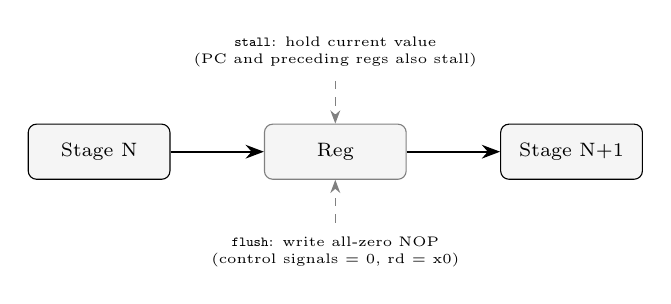
\begin{tikzpicture}[
        box/.style={draw, minimum width=1.8cm, minimum height=0.7cm,
                    font=\scriptsize, fill=pipeboxbg, rounded corners=3pt},
        arr/.style={-Stealth, thick}
      ]
        \node[box] (a) at (0,0) {Stage N};
        \node[box, draw=black!50] (r) at (3,0) {Reg};
        \node[box] (b) at (6,0) {Stage N+1};

        \draw[arr] (a) -- (r);
        \draw[arr] (r) -- (b);

        \node[font=\tiny, above=0.6cm of r, align=center]
          {\texttt{stall}: hold current value\\(PC and preceding regs also stall)};
        \node[font=\tiny, below=0.6cm of r, align=center]
          {\texttt{flush}: write all-zero NOP\\(control signals = 0, rd = x0)};

        \draw[-Stealth, dashed, gray] (3, 0.9) -- (r.north);
        \draw[-Stealth, dashed, gray] (3,-0.9) -- (r.south);
      \end{tikzpicture}

      \vspace{0.5em}
      \small
      \textbf{NOP encoding:} all-zero bits are a legal NOP (\texttt{ADDI x0, x0, 0}) because the opcode \texttt{0010011} with \texttt{rd=0} and \texttt{reg\_write=0} produces no visible side-effect.

      \vspace{0.4em}
      \begin{alertblock}{Priority rule}
        \small
        \textbf{Stall takes priority over flush.} If both are asserted simultaneously (e.g.\ load-use on a branch), stall wins to avoid losing the instruction in ID.
      \end{alertblock}
    \end{column}
  \end{columns}
\end{frame}

% ── hazard_unit ──────────────────────────────────────────────────────────────
\begin{frame}[fragile]{\texttt{hazard\_unit} --- Hazard Detection and Control}
  \begin{columns}[T]
    \begin{column}{0.52\textwidth}
      \textbf{Function}\\
      Detects the two structural hazard conditions that cannot be resolved by forwarding alone, and generates stall/flush signals for the pipeline registers and PC.

      \vspace{0.5em}
      \textbf{Load-use hazard detection}
      \begin{enumerate}\small
        \item Instruction in EX is a load (\texttt{ex\_mem\_read})
        \item Its destination (\texttt{ex\_rd}) matches rs1 or rs2 of the instruction in ID
        \item \texttt{ex\_rd != x0}
      \end{enumerate}
      \textbf{Action:} stall PC + IF/ID; flush ID/EX (NOP bubble)

      \vspace{0.5em}
      \textbf{Control hazard detection}\\
      EX stage resolves a taken branch (\texttt{branch\_taken}) or unconditional jump (\texttt{jump}).\\
      \textbf{Action:} flush IF/ID and ID/EX; redirect PC to target

      \vspace{0.5em}
      \small All outputs are \textbf{purely combinational} --- no latency added.
    \end{column}
    \begin{column}{0.44\textwidth}
\begin{lstlisting}
module hazard_unit (
  input  wire       ex_mem_read,
  input  wire [4:0] ex_rd,
  input  wire [4:0] id_rs1,
  input  wire [4:0] id_rs2,
  input  wire       branch_taken,
  input  wire       jump,
  output wire       pc_stall,
  output wire       if_id_stall,
  output wire       if_id_flush,
  output wire       id_ex_flush
);
  wire load_use =
    ex_mem_read &&
    (ex_rd != 5'b0) &&
    ((ex_rd == id_rs1) ||
     (ex_rd == id_rs2));

  wire redirect =
    branch_taken || jump;

  assign pc_stall    = load_use;
  assign if_id_stall = load_use;
  assign if_id_flush = redirect
                       && !load_use;
  assign id_ex_flush = load_use
                       || redirect;
endmodule
\end{lstlisting}
    \end{column}
  \end{columns}
\end{frame}

% ── forward_unit ─────────────────────────────────────────────────────────────
\begin{frame}[fragile]{\texttt{forward\_unit} --- Operand Forwarding}
  \begin{columns}[T]
    \begin{column}{0.52\textwidth}
      \textbf{Function}\\
      Detects RAW hazards that \emph{can} be resolved without a stall and generates 2-bit mux-select signals for the ALU input muxes in the EX stage.

      \vspace{0.5em}
      \textbf{Forwarding paths}

      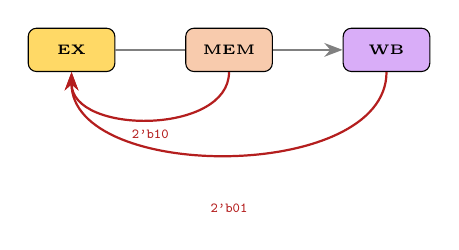
\begin{tikzpicture}[
        st/.style={draw, fill=#1, rounded corners=3pt, minimum width=1.1cm,
                   minimum height=0.55cm, font=\tiny\bfseries},
        arr/.style={-Stealth, thick, janusred}
      ]
        \node[st=stageEX]  (EX)  at (0,0)   {EX};
        \node[st=stageMEM] (MEM) at (2,0)   {MEM};
        \node[st=stageWB]  (WB)  at (4,0)   {WB};
        \draw[-Stealth, gray, thick] (EX)--(MEM)--(WB);
        % Forward arrows
        \draw[arr] (MEM.south) .. controls +(0,-0.8) and +(0,-0.8) .. (EX.south)
          node[midway, below, font=\tiny] {\texttt{2'b10}};
        \draw[arr] (WB.south) .. controls +(0,-1.4) and +(0,-1.4) .. (EX.south)
          node[midway, below, font=\tiny, yshift=-0.5cm] {\texttt{2'b01}};
      \end{tikzpicture}

      \vspace{0.3em}
      \textbf{Priority:} EX/MEM forwarding (\texttt{2'b10}) wins over MEM/WB (\texttt{2'b01}) when both match --- ensures the \emph{most recent} write is used.

      \vspace{0.3em}
      \textbf{Guard condition:} \texttt{rd != x0} must hold --- writing \texttt{x0} should not be forwarded.
    \end{column}
    \begin{column}{0.44\textwidth}
\begin{lstlisting}
// Forward A select
always @(*) begin
  if (mem_reg_write &&
      mem_rd != 5'b0 &&
      mem_rd == ex_rs1)
    forward_a = 2'b10; // EX/MEM
  else if (wb_reg_write &&
      wb_rd != 5'b0 &&
      wb_rd == ex_rs1)
    forward_a = 2'b01; // MEM/WB
  else
    forward_a = 2'b00; // regfile
end
// (mirror logic for forward_b)
\end{lstlisting}
      \vspace{0.4em}
      \begin{block}{ALU input mux (in \texttt{cpu.v})}
\begin{lstlisting}[basicstyle=\ttfamily\tiny]
wire [31:0] ex_rs1_data =
  (forward_a == 2'b10) ?
    mem_alu_result :
  (forward_a == 2'b01) ?
    wb_rd_data :
    ex_rs1_data_raw;
\end{lstlisting}
      \end{block}
    \end{column}
  \end{columns}
\end{frame}

% =============================================================================
\section{Phase 3 Extensions (Stretch Goals)}
% =============================================================================

\begin{frame}{Phase 3: Stretch Goal Options}
  \begin{columns}[T]
    \begin{column}{0.32\textwidth}
      \begin{block}{A --- Static Branch Prediction}
        \textbf{Strategy:} Backward-Taken, Forward-Not-Taken (BTFNT)\\[0.4em]
        Backward branches (negative offset) are predicted taken; forward branches are predicted not-taken.\\[0.4em]
        \textbf{Implement:}
        \begin{itemize}\scriptsize
          \item Predict at the end of IF using the sign bit of the B-type immediate
          \item On misprediction, flush and redirect
          \item Measure misprediction rate on benchmark programs
        \end{itemize}
      \end{block}
    \end{column}
    \begin{column}{0.32\textwidth}
      \begin{block}{B --- Direct-Mapped I-Cache}
        \textbf{Spec:} 256 entries, 4-byte lines (one word per line)\\[0.4em]
        Sits between \texttt{pc\_reg} and \texttt{imem}; hit serves the instruction in the same cycle. On a miss, the pipeline stalls while the cache fetches from ROM.\\[0.4em]
        \textbf{Implement:}
        \begin{itemize}\scriptsize
          \item Valid bit + tag per entry
          \item Stall PC and IF/ID on miss
          \item Report hit rate vs.\ benchmark
        \end{itemize}
      \end{block}
    \end{column}
    \begin{column}{0.32\textwidth}
      \begin{block}{C --- Basic Trap Handling}
        \textbf{CSRs required:}\\
        \texttt{mstatus}, \texttt{mtvec}, \texttt{mepc}, \texttt{mcause}\\[0.4em]
        Support \texttt{ECALL}, \texttt{EBREAK}, and \texttt{MRET}.\\[0.4em]
        \textbf{On trap:}
        \begin{enumerate}\scriptsize
          \item Save PC $\to$ \texttt{mepc}
          \item Set \texttt{mcause}
          \item Flush pipeline
          \item Jump to \texttt{mtvec}
        \end{enumerate}
        \textbf{On MRET:} restore PC from \texttt{mepc}
      \end{block}
    \end{column}
  \end{columns}
\end{frame}

% =============================================================================
\section{Verification and Toolflow}
% =============================================================================

\begin{frame}{Verification Strategy}
  \begin{columns}[T]
    \begin{column}{0.50\textwidth}
      \textbf{Test levels}
      \begin{enumerate}
        \item \textbf{Unit tests} --- each module in isolation\\
          e.g.\ drive all 11 ALU operations, check \texttt{result} and \texttt{zero}
        \item \textbf{Integration tests} --- short instruction sequences\\
          e.g.\ load-use sequence, branch-taken sequence
        \item \textbf{Compliance tests} --- \texttt{riscv-arch-test rv32i} suite\\
          Mandatory after Phase 2; covers all 47 instructions with edge cases
      \end{enumerate}

      \vspace{0.6em}
      \textbf{Pass/Fail protocol (testbench)}\\
      The test program stores a sentinel value to address \texttt{0xFFFF\_0000}:
      \begin{itemize}\small
        \item \texttt{SW x1, 0(magic)} where \texttt{x1 = 1} $\Rightarrow$ \textbf{PASS}
        \item \texttt{SW x0, 0(magic)} $\Rightarrow$ \textbf{FAIL}
      \end{itemize}
      The testbench monitors this address and calls \texttt{\$finish}.
    \end{column}
    \begin{column}{0.46\textwidth}
      \textbf{Toolflow}
      \begin{enumerate}\small
        \item Write assembly test: \texttt{test.s}
        \item Assemble:\\
          \texttt{riscv64-unknown-elf-as}\\
          \texttt{\ \ -march=rv32i -mabi=ilp32}\\
          \texttt{\ \ -o test.o test.s}
        \item Link and extract hex:\\
          \texttt{riscv64-unknown-elf-ld -o test.elf test.o}\\
          \texttt{riscv64-unknown-elf-objcopy}\\
          \texttt{\ \ -O verilog test.elf prog.hex}
        \item Simulate:\\
          \texttt{verilator --binary -j0 tb\_top.v}\\
          \texttt{./obj\_dir/Vtb\_top}
        \item View waveforms:\\
          \texttt{gtkwave dump.vcd}
      \end{enumerate}

      \begin{exampleblock}{Tip}
        \small
        Use \texttt{make} to automate the assemble $\to$ simulate pipeline; one target per test case keeps iteration fast.
      \end{exampleblock}
    \end{column}
  \end{columns}
\end{frame}

% ── Grading ──────────────────────────────────────────────────────────────────
\begin{frame}{Grading Rubric \& Timeline}
  \begin{columns}[T]
    \begin{column}{0.45\textwidth}
      \begin{block}{Grading (100 points)}
        \renewcommand{\arraystretch}{1.2}
        \begin{tabular}{lc}
          \toprule
          Component & Points \\
          \midrule
          Phase 1: Single-cycle datapath & 35 \\
          Phase 2: Pipeline registers + forwarding & 30 \\
          Phase 2: Stall and flush logic & 20 \\
          Phase 3: One stretch goal & 10 \\
          Code quality \& documentation & 5 \\
          \midrule
          \textbf{Total} & \textbf{100} \\
          \bottomrule
        \end{tabular}
      \end{block}
    \end{column}
    \begin{column}{0.50\textwidth}
      \begin{block}{4-Week Timeline}
        \renewcommand{\arraystretch}{1.2}
        \begin{tabular}{lp{5.2cm}}
          \toprule
          Week & Milestone \\
          \midrule
          1 & All Phase 1 modules complete; unit tests passing \\
          2 & Pipeline registers added; basic instruction sequences verified \\
          3 & Forwarding and hazard units complete; Phase 2 tests passing \\
          4 & One Phase 3 extension done; riscv-arch-test passing; write-up submitted \\
          \bottomrule
        \end{tabular}
      \end{block}
    \end{column}
  \end{columns}
\end{frame}

% =============================================================================
\section{Summary}
% =============================================================================

\begin{frame}{Key Takeaways}
  \begin{columns}[T]
    \begin{column}{0.48\textwidth}
      \textbf{ISA}
      \begin{itemize}
        \item RV32I: 47 instructions, 6 encoding formats, fixed 32-bit width
        \item opcode selects the class; funct3/funct7 select the variant
        \item \texttt{x0} is always zero; \texttt{pc} is not directly addressable
        \item Branch and jump targets are PC-relative (B, J types) or register-relative (JALR)
      \end{itemize}

      \vspace{0.6em}
      \textbf{Single-cycle datapath}
      \begin{itemize}
        \item Five stages, all combinational, one clock per instruction
        \item Two-level control decode: \texttt{ctrl} $\to$ \texttt{alu\_ctrl}
        \item Harvard memory: separate \texttt{imem} and \texttt{dmem}
        \item Clock period bounded by the critical (load) path
      \end{itemize}
    \end{column}
    \begin{column}{0.48\textwidth}
      \textbf{5-stage pipeline}
      \begin{itemize}
        \item Four pipeline registers separate the five stages
        \item Hazards are unavoidable; manage them explicitly
        \item Forwarding eliminates most RAW stalls
        \item Load-use requires one stall cycle (no forwarding possible)
        \item Branch penalty: 2 cycles (predict-not-taken + flush on taken)
      \end{itemize}

      \vspace{0.6em}
      \textbf{Module responsibilities (one module, one job)}
      \begin{itemize}
        \item \texttt{hazard\_unit}: stall/flush signals only
        \item \texttt{forward\_unit}: mux-select signals only
        \item \texttt{ctrl}: control signals from opcode only
        \item \texttt{alu\_ctrl}: ALU op from alu\_op + funct3/7 only
      \end{itemize}
    \end{column}
  \end{columns}

  \vspace{0.6em}
  \begin{center}
    \large\textbf{Good luck! Start with Phase 1, test early, test often.}
  \end{center}
\end{frame}

% ── Final slide ───────────────────────────────────────────────────────────────
\begin{frame}
  \begin{center}
    \vspace{1.5em}
    {\Large\textbf{Questions?}}\\[1.5em]
    \large Janus Lab --- CPU Design and Implementation\\[0.5em]
    \normalsize Lecture 01: RISC-V ISA, Microarchitecture, and Module Overview\\[2em]
    \small
    \begin{tabular}{ll}
      Spec:      & \texttt{docs/spec.md} \\
      Source:    & \texttt{cpu/*.v} \\
      Testbench: & \texttt{cpu/tb\_top.v} \\
      Tests:     & \texttt{tests/phase\{1,2,3\}/} \\
    \end{tabular}
  \end{center}
\end{frame}

\end{document}
